\tikzsetnextfilename{figures/metricas/figure}
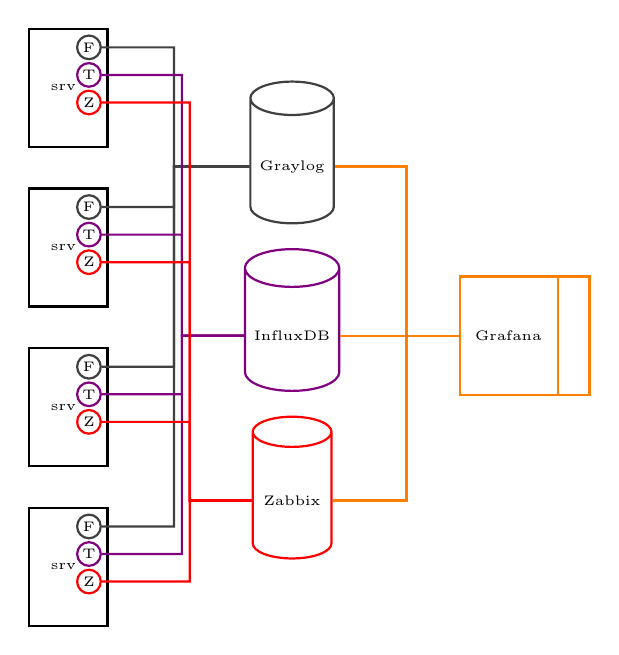
\begin{tikzpicture}[
    font=\tiny,
    thick
  ]
\usetikzlibrary{positioning,fit,calc,shapes}
\def\nw{1cm}

\tikzstyle{bignode}=[minimum height=1.5*\nw,minimum width=\nw,node distance=.5*\nw];

\node[draw,bignode] (srv1) {srv\,\,\,};
\node[draw,bignode,below= of srv1] (srv2) {srv\,\,\,};
\node[draw,bignode,below= of srv2] (srv3) {srv\,\,\,};
\node[draw,bignode,below= of srv3] (srv4) {srv\,\,\,};


\tikzstyle{agent}=[circle,draw,minimum height=.3*\nw,minimum width=.3*\nw,inner sep=0mm];
\tikzstyle{g}=[draw=darkgray];
\node[agent,g] at ($ (srv1.north east) - (.25*\nw,.25*\nw) $) (f1) {F};
\node[agent,g] at ($ (srv2.north east) - (.25*\nw,.25*\nw) $) (f2) {F};
\node[agent,g] at ($ (srv3.north east) - (.25*\nw,.25*\nw) $) (f3) {F};
\node[agent,g] at ($ (srv4.north east) - (.25*\nw,.25*\nw) $) (f4) {F};

\tikzstyle{t}=[draw=violet];
\node[agent,t] at ($ (srv1.north east) - (.25*\nw,.6*\nw) $) (t1) {T};
\node[agent,t] at ($ (srv2.north east) - (.25*\nw,.6*\nw) $) (t2) {T};
\node[agent,t] at ($ (srv3.north east) - (.25*\nw,.6*\nw) $) (t3) {T};
\node[agent,t] at ($ (srv4.north east) - (.25*\nw,.6*\nw) $) (t4) {T};

\tikzstyle{zbx}=[draw=red];
\node[agent,zbx] at ($ (srv1.north east) - (.25*\nw,.95*\nw) $) (z1) {Z};
\node[agent,zbx] at ($ (srv2.north east) - (.25*\nw,.95*\nw) $) (z2) {Z};
\node[agent,zbx] at ($ (srv3.north east) - (.25*\nw,.95*\nw) $) (z3) {Z};
\node[agent,zbx] at ($ (srv4.north east) - (.25*\nw,.95*\nw) $) (z4) {Z};

\coordinate (aux0) at ($ (srv1) - (-2*\nw,\nw) $);

\tikzstyle{server}=[cylinder,bignode,minimum height=1.8*\nw, node distance=0.3*\nw,shape border rotate=90, shape aspect=0.4];
\node[g,server, right = of aux0] (graylog) {Graylog};
\node[t,server, below= of graylog] (influxdb) {InfluxDB};
\node[zbx,server, below= of influxdb] (zabbix) {Zabbix};

\node[draw=orange,bignode,rectangle split,rectangle split horizontal,rectangle split parts=2, node distance=1.5*\nw,text width=\nw,align=center,right = of influxdb] (grafana) {Grafana};

\coordinate (auxg) at ($ (graylog) - (1.5*\nw,0) $);

% \node[fit=(srv1.north west)(srv3.south west)(graylog.east),draw,dashed] (ex) {};
% \node[] at ($ (ex.south east) + (-1.7*\nw,.3*\nw) $) {{infraestructura existente}};

\draw[-,g] (f1) -| (auxg) -- (graylog.west);
\draw[-,g] (f2) -| (auxg) -- (graylog.west);
\draw[-,g] (f3) -| (auxg) -- (graylog.west);
\draw[-,g] (f4) -| (auxg) -- (graylog.west);

\coordinate (auxi) at ($ (influxdb) - (1.5*\nw-0.1cm,0) $);
\draw[-,t] (t1) -| (auxi) -- (influxdb.west);
\draw[-,t] (t2) -| (auxi) -- (influxdb.west);
\draw[-,t] (t3) -| (auxi) -- (influxdb.west);
\draw[-,t] (t4) -| (auxi) -- (influxdb.west);

\coordinate (auxz) at ($ (zabbix) - (1.5*\nw-0.2cm,0) $);
\draw[-,zbx] (z1) -| (auxz) -- (zabbix.west);
\draw[-,zbx] (z2) -| (auxz) -- (zabbix.west);
\draw[-,zbx] (z3) -| (auxz) -- (zabbix.west);
\draw[-,zbx] (z4) -| (auxz) -- (zabbix.west);

\coordinate (auxgra) at ($ (grafana) - (1.5*\nw,0) $);
\draw[-,draw=orange] (graylog.east) -| (auxgra) -- (grafana.west);
\draw[-,draw=orange] (influxdb.east) -| (auxgra) -- (grafana.west);
\draw[-,draw=orange] (zabbix.east) -| (auxgra) -- (grafana.west);


% \draw[-,draw] (logserver) -- (graylog.west);

% \node[below=of logserver] (ssh) {Acceso ssh};
% \node[below=of graylog] (web) {Acceso web};
% 
% \draw[-stealth] (ssh) -- (graylog.south);
% \draw[-stealth] (web) -- (graylog.south);

\end{tikzpicture}
